\section{网络层}
\subsection{组播}
\subsubsection{组播地址}

组播报文的目的地址使用D类IP地址, D类地址不能出现在IP报文的源IP地址字段。

单播数据传输过程中,一个数据包传输的路径是从源地址路由到目的地址,利用“逐跳”的原理在IP网络中传输。

然而在ip组播环中,数据包的目的地址不是一个,而是一组,形成组地址。

所有的信息接收者都加入到一个组内,并且一旦加入之后,流向组地址的数据立即开始向接收者传输,组中的所有成员都能接收到数据包。
组播组中的成员是动态的,主机可以在任何时刻加入和离开组播组。

\subsubsection{范围}

\begin{itemize}
    \item 224.0.0.0~224.0.0.255为预留的组播地址(永久组地址),地址224.0.0.0保留不做分配,其它地址供路由协议使用;
    \item 224.0.1.0~224.0.1.255是公用组播地址,可以用于Internet;
    \item 224.0.2.0~238.255.255.255为用户可用的组播地址(临时组地址),全网范围内有效;
    \item 239.0.0.0~239.255.255.255为 \textbf{本地} 管理组播地址,仅在特定的本地范围内有效。

\end{itemize}

\subsubsection{组播IP地址和MAC地址转换}

组播MAC地址有IP地址映射转换而成,过程如下图所示:

\begin{figure}[ht]
    \centering
    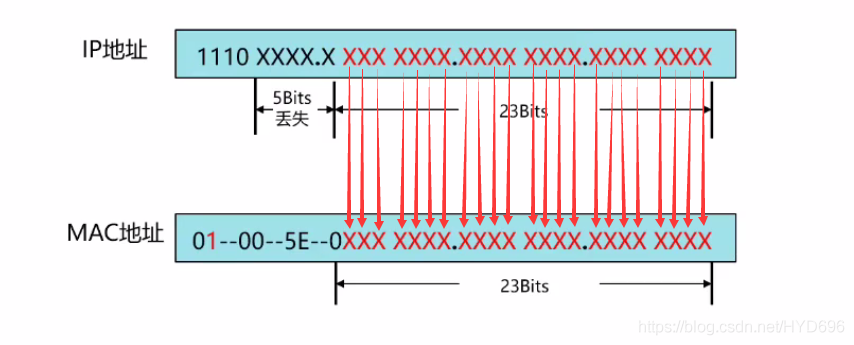
\includegraphics[scale=0.7]{pic/multicast-01.png}
    \caption{multicast ip addr to mac}
    \label{fig:multicast_ip_addr_to_mac}
\end{figure}


过程如下:

\begin{enumerate}
    \item 加上MAC地址固定前缀(24bit)为:01-00-5E;
    \item 后面24bit由IP地址的后23bit构成;
    \item 第25 bit位固定为0;
\end{enumerate}

\subsubsection{举例}

以Someip SD服务组播地址为例,组播IP地址为 \textbf{239.127.3.1}。

\begin{itemize}
    \item 二进制: \textbf{1110 1111 0111 1111 0000 0011 0000 0001}
    \item 固定前缀: \textbf{01-00-5E- + 0b}
    \item 转换结果: \textbf{01-00-5e-7f-03-01}
\end{itemize}

\subsubsection{代码实现}

协议栈中由TCPIP模块分配多播IP地址到设置 \lstinline{ENET} multicast mac filter \lstinline{ENETn_GAUR/GALR}寄存器的过程如下图所示:

\begin{figure}[h]
    \centering
    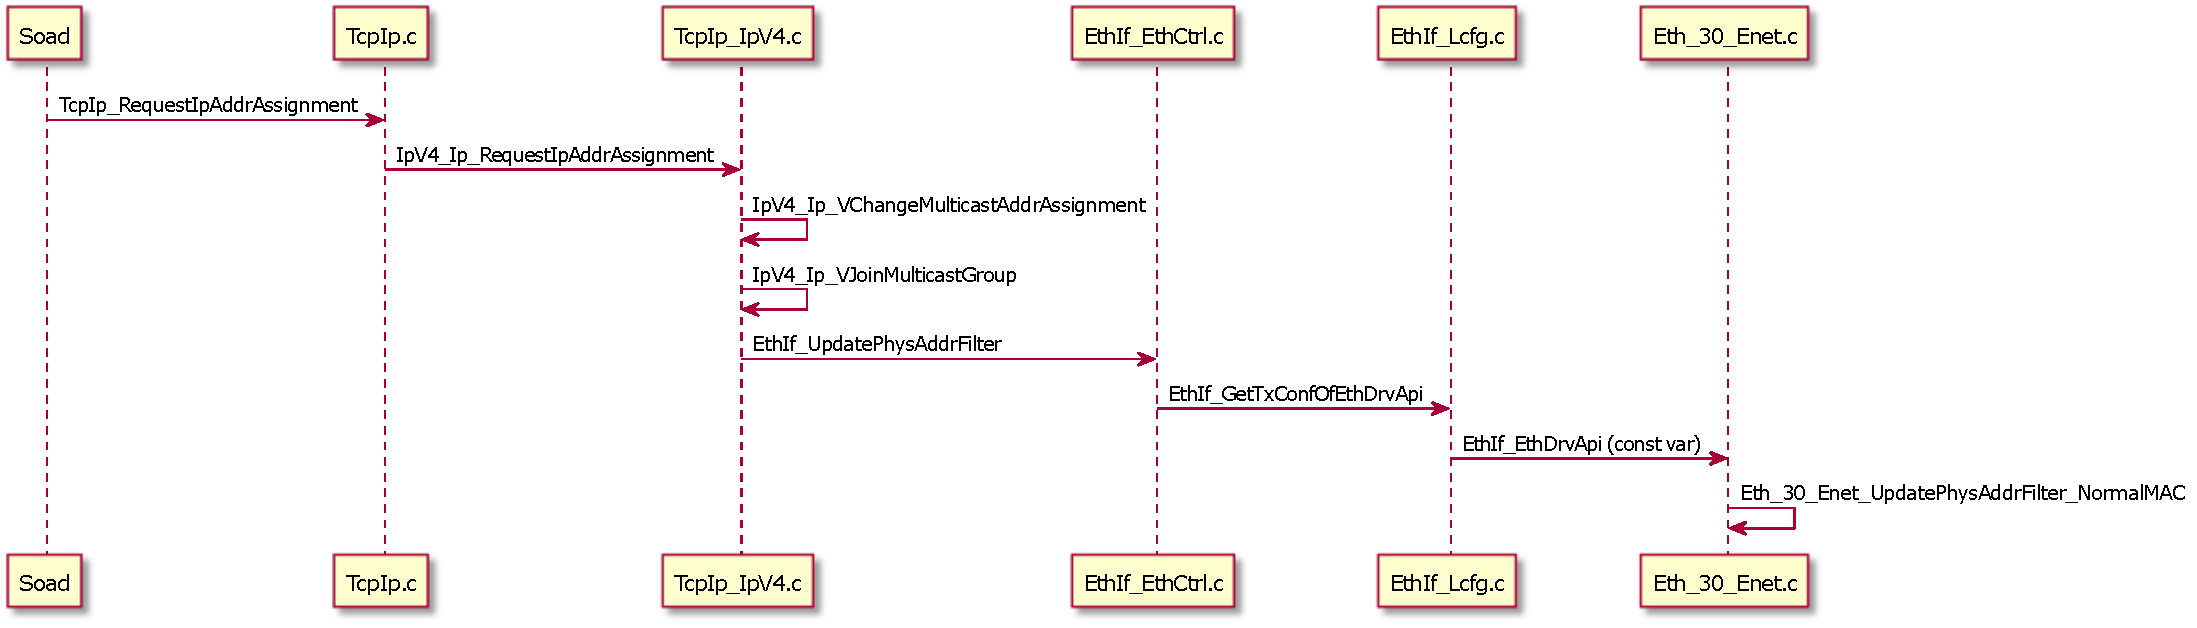
\includegraphics[scale=0.5]{pic/eth_multicast_mac_code.pdf}
    \caption{eth multicast mac code}
    \label{fig:eth_multicast_mac_code}
\end{figure}